\section{OPC UA}

\subsection{What is OPC UA?}

OPC UA is an open and royalty free set of standards designed as a universal factory floor communications protocol.
OPC UA is designed specifically for the factory and industrial environment. While there are numerous communication solutions available, OPC UA has several advantages:

\begin{itemize}
\item A state of art security model (see [UA Part 2]).
\item A fault tolerant communication protocol.
\item An information modeling framework that allows application developers to represent their data in a way that makes sense to them.
\end{itemize}

OPC UA has a broad scope which delivers for economies of scale for application developers. This means that a larger number of high quality applications at a reasonable cost are available to factory owners. When combined with powerful semantic models such as MTConnect, OPC UA makes it easier for factory owners to access data via generic commercial application.

The OPC UA model is scalable from small devices to ERP systems. OPC UA devices process information locally and then provide that data in a consistent format to any application requesting data - ERP, MES, PMS, Maintenance Systems, HMI, Smartphone or a standard Browser, for examples. For a more complete overview see [UA Part 1].

\subsection{Basics of OPC UA}

As an Open Standard, OPC UA is based on standard Internet technologies – TCP/IP, HTTP, Ethernet, and XML.

As an Extensible Standard, OPC UA provides a set of services (see [UA Part 4]) and a basic information model framework. This framework provides an easy manner for creating and exposing vendor defined information in a standard way. More importantly all OPC UA Clients are expected to be able to discover and use vendor defined information. This means OPC UA users can benefit from the economies of scale that come with generic visualization and historian applications. This specification is an example of an OPC UA Information Model designed to meet the needs of Machine Tool developers and users.

OPC UA Clients can be any consumer of factory data from another device on the network to browser base thin clients and ERP systems. The full scope of OPC UA applications are shown in Figure \ref{fig:scope_of_opcua}.

The services are described in the following service sets:
\begin{itemize}
\item Discovery Service Set -- used by a Client to discover the Servers and connection information that are available in a system
\item Secure Channel Service Set -- used to establish secure communication over which all subsequent communication occurs. Secure channels specify communication protocols and encoding of data. They are used in conjunction with Session Services and provide consistent functionality for all service sets irrespective of the selected communication protocol (TCP, HTTP, HTTPs) data Encoding (OPC Binary, XML) or network architecture (firewalls, routers \ldots). 
\item Session Service Set -- is used to establish a session context that is used for subsequent communication, including user information. This session context is not lost if a communication error occurs , allowing secure channels to be recovered or rebuilt without data loss
\item \texttt{NodeManagement} Service Set -- allows clients to manage the \texttt{AddressSpace} available in a Server where the \texttt{AddressSpace} is all of the Nodes, both instance and type definition and all of the relationships between them. Management includes adding / deleting nodes and adding / deleting relationships between nodes. Not all Servers support node management functionality.
\item View Service Set – used by a Client to discover the information model that is being exposed in the \texttt{AddressSpace} of the Server It include simple browsing of the address space, but also include services to cover browse information to concrete node references (\texttt{NodeIds})
\item Query Service Set -- is an extension to view service allowing a client to query the \texttt{AddressSpace} of large servers. Usually on large servers support Query services 
\item Attribute Service Set -- allows a client to read and write current and historical values to nodes in the address spaces.
\item Method Service Set -- allow Servers to extend the functionality provided by a system, without having to define new services. The methods are defined in the \texttt{AddressSpace} as part of an information model. Client can discover the available methods using the View Service Set and access them via this service set.
\item \texttt{MonitoredItem} Service Set -- used by client in conjunction with the Subscription Service Set to obtain a steady stream of values. This Service Set allows the client to define the individual data that is to be reported, filters and buffering for the items and the sampling rate.
\item Subscription Service Set -- used by the client in conjunction with the \texttt{Monitored\-Item} Service Set to obtain a steady stream of values. This service set is used to define the grouping of items to be returned and the interval at which they are sent.
\end{itemize}

These standard services are available with any information model, allowing for generic Client access to any Server.

\begin{figure}[h]
  \centering
  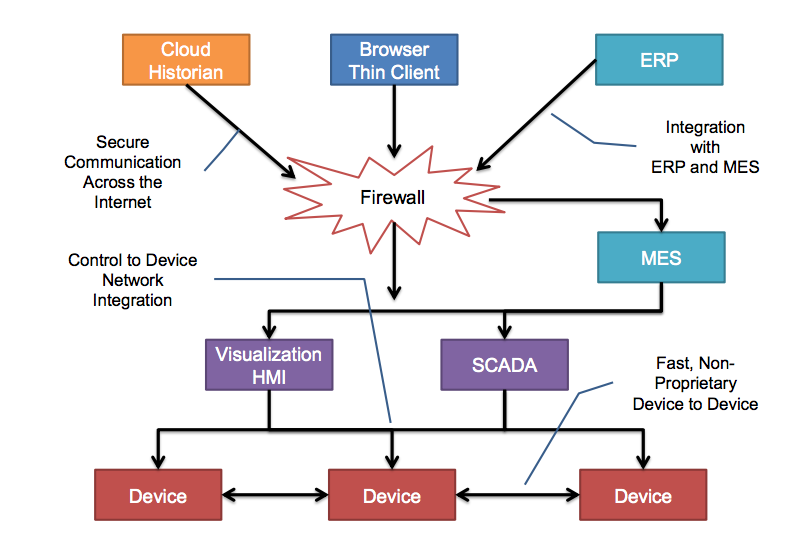
\includegraphics[width=0.85\textwidth]{diagrams/ScopeOfOpcUAEnt.png}
  \caption{The Scope of OPC UA within an Enterprise }
  \label{fig:scope_of_opcua}
\end{figure}

\subsection{Information Modeling in OPC UA}

\subsubsection{Concepts}

OPC UA provides a framework that can be used to represent complex information as Objects in an address space which can be accessed with standard web services. These Objects consist of Nodes connected by References. Different classes of Nodes convey different semantics. For example a Variable Node represents a value that can be read or written. The Variable Node has an associated \texttt{DataType} that can define the actual value, such as a string, float, structure etc. It can also describe the variable value as a variant. A Method Node represents a function that can be called. Every Node has a number of Attributes including a unique identifier called a \texttt{NodeId} and non-localized name called as \texttt{BrowseName}. All of these concepts combined together create what is commonly reference to in OPC UA as the Address Spssace. An Object representing a 'Reservation' is shown in Figure \ref{fig:opcua_basic_object} as an illustration of these concepts.

\begin{quote}
\footnotesize
NOTE: The figures used to illustrate OPC UA information models use a notation that was developed for the OPC UA specification. The notation is summarized in Figure \ref{fig:opc_ua_notation}. UML representations can also be used; however, the OPC UA notation is less ambiguous because there is a direct mapping from the elements in the figures to Nodes in the address space of an OPC UA server. A complete description of the different types of Nodes and References can be found in [UA Part 3] and the base OPC UA Address space is described in [UA Part 5].
\end{quote}

\begin{figure}[h]
  \centering
  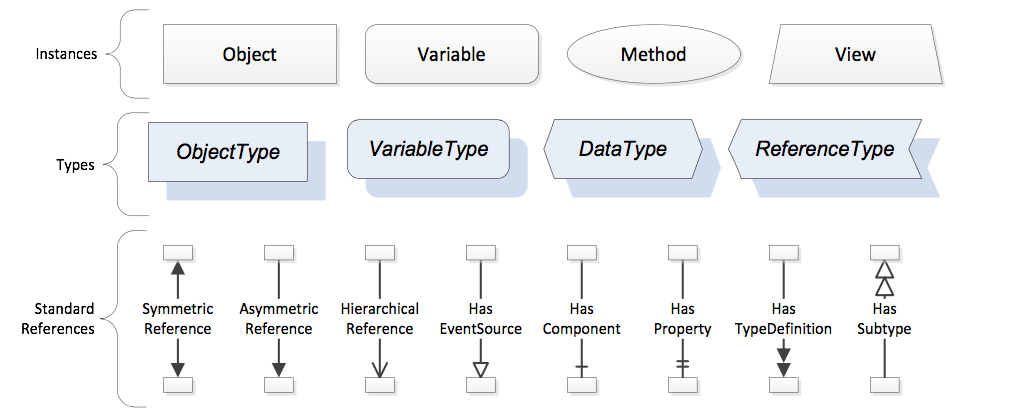
\includegraphics[width=1.0\textwidth]{diagrams/OpcInfoModelNotation.png}
  \caption{The OPC UA Information Model Notation}
  \label{fig:opc_ua_notation}
\end{figure}

\begin{figure}[h]
  \centering
  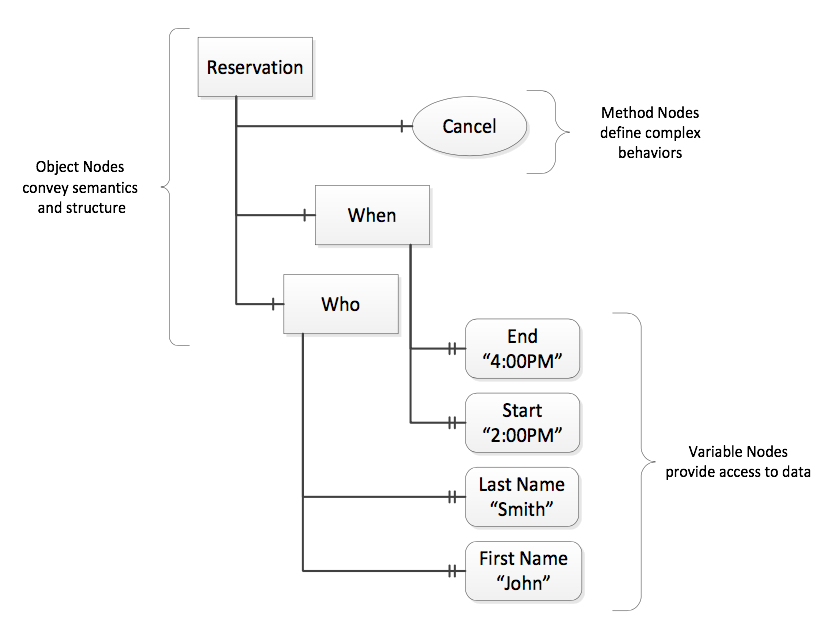
\includegraphics[width=1.0\textwidth]{diagrams/OpcUaBasicObject.png}
  \caption{A Basic Object in an OPC UA Address Space}
  \label{fig:opcua_basic_object}
\end{figure}

\texttt{Object} and \texttt{Variable Nodes} are called \texttt{Instance Nodes} and they always reference a Type Definition (\texttt{ObjectType} or \texttt{VariableType}) Node which describes their semantics and structure. Figure \ref{fig:rel_type_inst} illustrates the relationship between an Instance and its Type Definition.

The Type Nodes are templates that define all of the children that can be present in an Instance of the Type. In the example in Figure \ref{fig:rel_type_inst} the \texttt{PersonType} \texttt{ObjectType} defines two children: First Name and Last Name. All instances of \texttt{PersonTyp}e are expected to have the same children with the same \texttt{BrowseNames}. Within a Type the \texttt{BrowseNames} uniquely identify the child. This means Client applications can be designed to search for children based on the \texttt{BrowseNames} from the Type instead of \texttt{NodeIds}. This eliminates the need for manual reconfiguration of systems if a Client uses Types that multiple devices implement.

OPC UA also supports the concept of sub typing. This allows a modeler to take an existing Type and extend it. There are rules regarding sub typing defined in [UA Part 3], but in general they allow the additions to a given type or the restriction of a \texttt{DataType} to a more specific data type. For example the modeler may decide that the existing \texttt{ObjectType} in some cases needs an additional variable. The modeler can create a subtype of the \texttt{ObjectType} and add the variable. A client that is expecting the parent type can treat the new \texttt{ObjectType} as if it was of the parent \texttt{ObjectType} and just ignore the additional variable. A client that understands the new subtype may display or otherwise process the additional variable. With regard to \texttt{DataTypes}, if a variable is defined to have a numeric value, a sub type could restrict the Value to a float.

\begin{figure}[h]
  \centering
  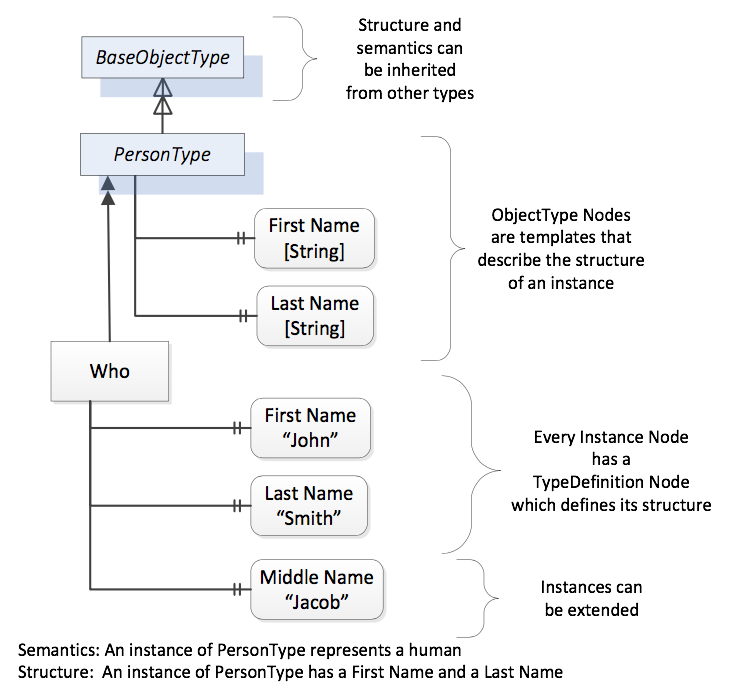
\includegraphics[width=1.0\textwidth]{diagrams/RelsBetweenTypesAndInstances.png}
  \caption{The Relationship between Type Definitions and Instances }
  \label{fig:rel_type_inst}
\end{figure}

References allow Nodes to be connected together in ways that describe their relationships. All References have a ReferenceType that specifies the semantics of the relationship. References can be hierarchical or non-hierarchical. Hierarchical references are used to create the structure of Objects and Variables. Non-hierarchical are used to create arbitrary associations. Applications can define their own ReferenceType by creating Subtypes of the existing ReferenceType. Subtypes inherit the semantics of the parent but may add additional restrictions. Figure \ref{fig:ref_bet_objs} depicts several references connecting different Objects.

\begin{figure}[h]
  \centering
  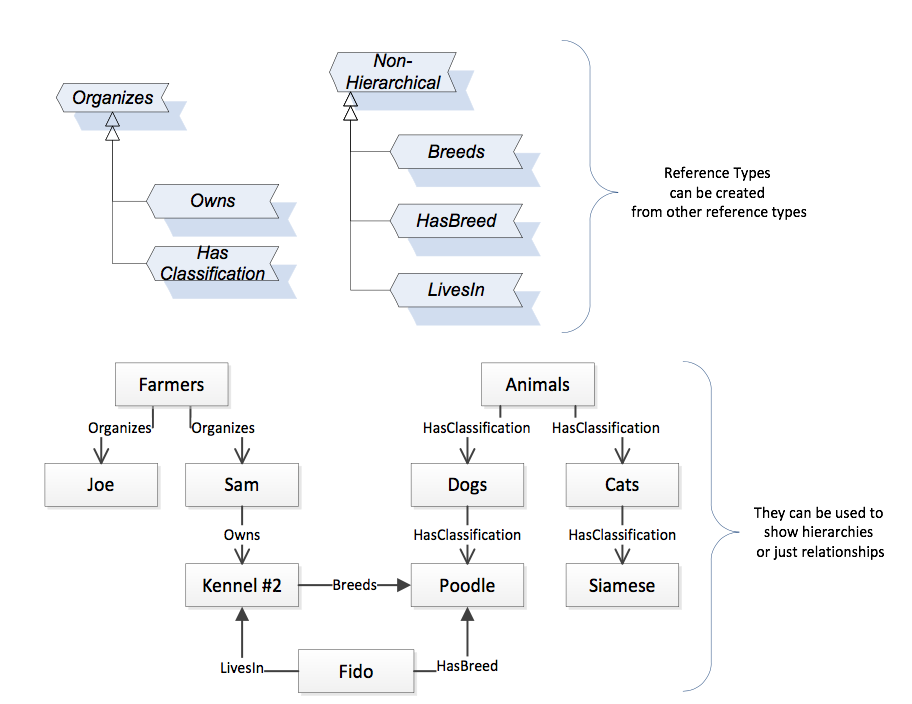
\includegraphics[width=1.0\textwidth]{diagrams/RefsBetweenObjects.png}
  \caption{Examples of References between Objects}
  \label{fig:ref_bet_objs}
\end{figure}

OPC UA specification defines a very wide range of functionality in its basic information model. It is not expected that all clients or servers support all functionality in the OPC UA specifications. OPC UA includes the concept of profiles, which segment the functionality into testable certifiable units. This allows the development of companion specification (such as MTConnect-OPC UA) that can describe the subset of functionality that is expected to be implemented. The profiles do not restrict functionality, but generate requirements for a minimum set of functionality (see [UA Part 7])

The OPC foundation also defines a set of information models that provide a basic set of functionality. The Data Access specification (see [UA Part 8]) provides a basic information model for typical data. The Alarm and Condition specification (see [UA Part 9]) defines a standard information model for Alarms and Conditions. The Programs specification (see [UA Part 10]) defines a stand information model for extending the functionality available via method calls and state machines. The Historical Access specification (see [UA Part 11]) defines the information model associated with Historical Data and Historical Events. The aggregates specification (see [UA Part 13]) defines a series of standard aggregate function that allow a client to request summary data. Examples of aggregates include averages, minimums, time in state, Standard deviation, etc. 

\subsubsection{Namespaces}

OPC UA allows information from many different sources to be combined into a single coherent address space. \texttt{Namespaces} are used to make this possible by eliminating naming and id conflicts between information from different sources. \texttt{Namespaces} in OPC UA have a globally unique string called a \texttt{NamespaceUri} and a locally unique integer called a \texttt{NamespaceIndex}. The \texttt{NamespaceIndex} is only unique within the context of a Session between an OPC UA Client and an OPC UA Server. All of the web services defined for OPC UA use the \texttt{NamespaceIndex} to specify the \texttt{Namespace} for qualified values.

There are two types of values in OPC UA that are qualified with Namespaces: \texttt{NodeIds} and \texttt{QualifiedNames}. \texttt{NodeIds} are globally unique identifiers for Nodes. This means the same Node with the same \texttt{NodeId} can appear in many Servers. This, in turn, means Clients can have built in knowledge of some Nodes. OPC UA Information Models generally define globally unique \texttt{NodeIds} for the \texttt{TypeDefinitions} defined by the Information Model.

\texttt{QualifiedNames} are non-localized names qualified with a \texttt{Namespace}. They are used for the \texttt{BrowseNames} of Nodes and allow the same Names to be used by different information models without conflict. The \texttt{BrowseName} is used to identify the children within a \texttt{TypeDefinitions}. Instances of a \texttt{TypeDefinition} are expected to have children with the same \texttt{BrowseNames}. \texttt{TypeDefinitions} are not allowed to have children with duplicate \texttt{BrowseNames}; however, Instances do not have that restriction.

\subsubsection{Companion Specifications}

An OPC UA companion specification for an industry specific vertical market describes an information model by defining ObjectTypes, VariableTypes, DataTypes and ReferenceTypes that represent the concepts used in the vertical market. Table \ref{table:ex_object_type_definition} contains an example of an ObjectType definition.

\begin{table}[ht]
\centering 
  \caption{Example \texttt{ObjectType} Definition}
  \label{table:ex_object_type_definition}
\fontsize{9pt}{11pt}\selectfont
\tabulinesep=3pt
\begin{tabu} to 6in {|l|l|l|l|l|l|} \everyrow{\hline}
\hline
\rowfont\bfseries {Attribute} & \multicolumn{5}{|l|}{Value} \\
\tabucline[1.5pt]{}
BrowseName & \multicolumn{5}{|l|}{WidgetType} \\
IsAbstract & \multicolumn{5}{|l|}{True} \\
\tabucline[1.5pt]{}
\rowfont \bfseries References & NodeClass & BrowseName & DataType & TypeDefinition & {Modeling Rule} \\
\multicolumn{6}{|l|}{Subtype of the BaseObjectType from [UA Part 5]} \\
HasProperty & Variable & Color &  String & PropertyType & Optional \\
HasProperty & Variable & Flavor &  Double & PropertyType & Mandatory \\
HasProperty & Variable & Rank &  Int32 & PropertyType & Mandatory \\
\end{tabu}
\end{table} 

The \texttt{BrowseName} is a non-localized name for an \texttt{ObjectType}. 

\texttt{IsAbstract} is a flag indicating whether instances of the \texttt{ObjectType} can be created.

The bottom of the table lists the child nodes for the type. The Reference is the type of reference between the Object instance and the child Node. The \texttt{NodeClass} is the class of Node. The \texttt{BrowseName} is the non-localized name for the child. The \texttt{DataType} is the structure of the Value accessible via the Node (only used for Variable \texttt{NodeClass} Nodes) and the \texttt{TypeDefinition} is the \texttt{ObjectType} or \texttt{VariableType} for the child. 

The \texttt{ModellingRule} indicates whether a child is Mandatory or Optional. It can also indicate cardinality. Note that the \texttt{BrowseName} is not defined if the cardinality is greater than 1. Figure \ref{fig:sample_object_type} visually depicts the \texttt{ObjectType} defined in Table \ref{table:ex_object_type_definition} along with two instances of the \texttt{ObjectType}.

\begin{figure}[h]
  \centering
  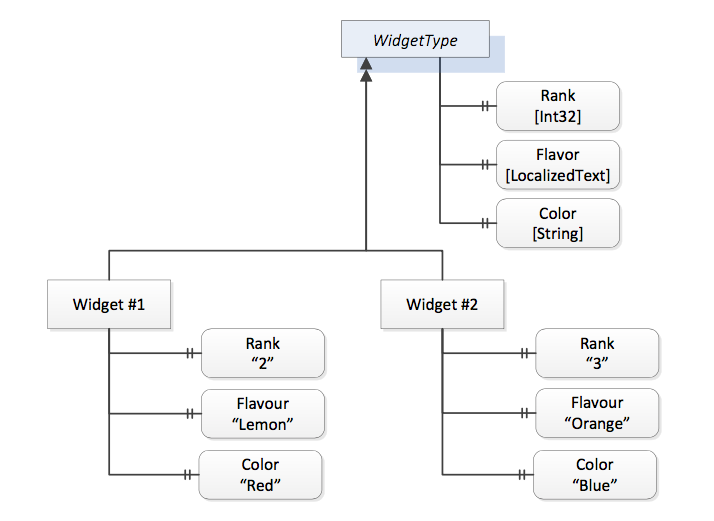
\includegraphics[width=1.0\textwidth]{diagrams/SampleObjectType.png}
  \caption{A Visual Representation of the Sample ObjectType}
  \label{fig:sample_object_type}
\end{figure}

\FloatBarrier

